
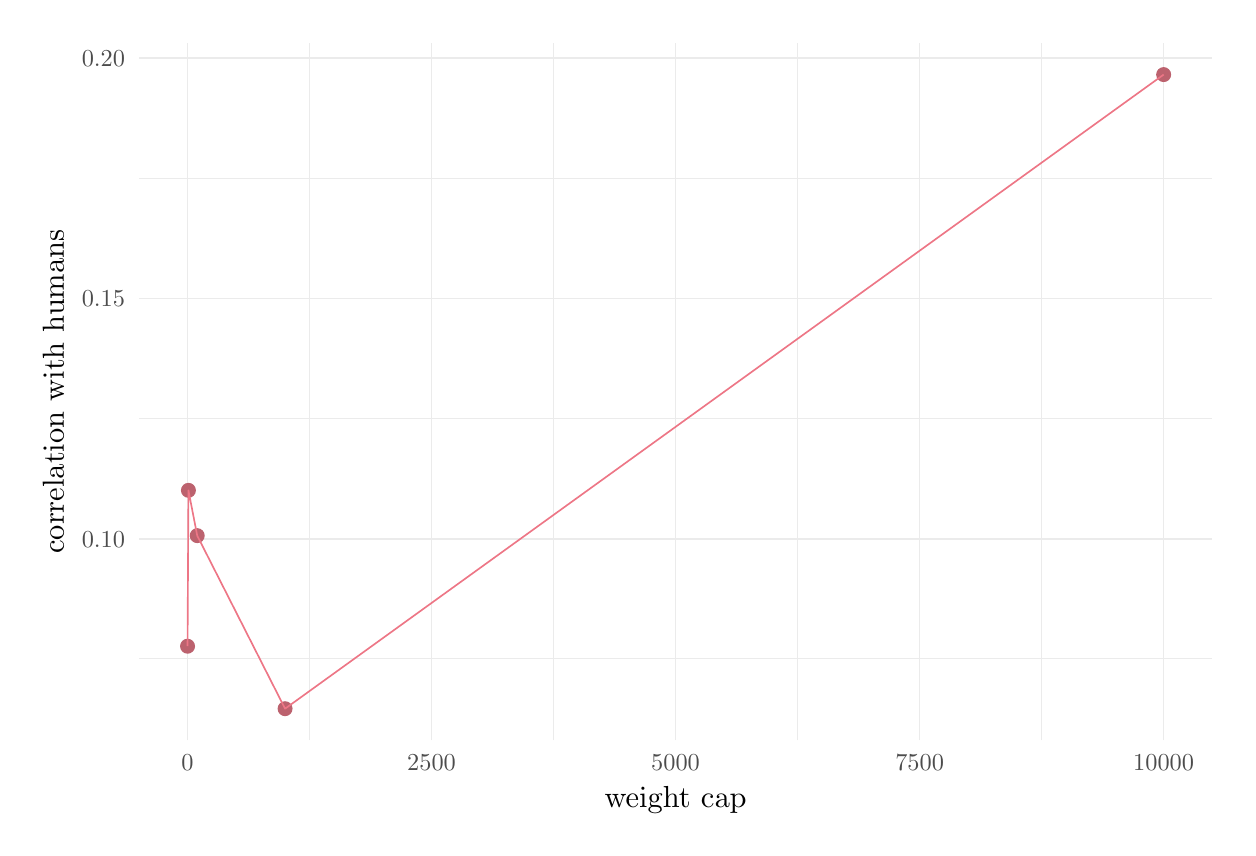
\begin{tikzpicture}[x=1pt,y=1pt]
\definecolor{fillColor}{RGB}{255,255,255}
\path[use as bounding box,fill=fillColor,fill opacity=0.00] (0,0) rectangle (433.62,289.08);
\begin{scope}
\path[clip] ( 40.14, 31.53) rectangle (428.12,283.58);
\definecolor{drawColor}{gray}{0.92}

\path[draw=drawColor,line width= 0.3pt,line join=round] ( 40.14, 60.99) --
	(428.12, 60.99);

\path[draw=drawColor,line width= 0.3pt,line join=round] ( 40.14,147.85) --
	(428.12,147.85);

\path[draw=drawColor,line width= 0.3pt,line join=round] ( 40.14,234.70) --
	(428.12,234.70);

\path[draw=drawColor,line width= 0.3pt,line join=round] (101.83, 31.53) --
	(101.83,283.58);

\path[draw=drawColor,line width= 0.3pt,line join=round] (190.02, 31.53) --
	(190.02,283.58);

\path[draw=drawColor,line width= 0.3pt,line join=round] (278.20, 31.53) --
	(278.20,283.58);

\path[draw=drawColor,line width= 0.3pt,line join=round] (366.39, 31.53) --
	(366.39,283.58);

\path[draw=drawColor,line width= 0.6pt,line join=round] ( 40.14,104.42) --
	(428.12,104.42);

\path[draw=drawColor,line width= 0.6pt,line join=round] ( 40.14,191.27) --
	(428.12,191.27);

\path[draw=drawColor,line width= 0.6pt,line join=round] ( 40.14,278.13) --
	(428.12,278.13);

\path[draw=drawColor,line width= 0.6pt,line join=round] ( 57.74, 31.53) --
	( 57.74,283.58);

\path[draw=drawColor,line width= 0.6pt,line join=round] (145.93, 31.53) --
	(145.93,283.58);

\path[draw=drawColor,line width= 0.6pt,line join=round] (234.11, 31.53) --
	(234.11,283.58);

\path[draw=drawColor,line width= 0.6pt,line join=round] (322.30, 31.53) --
	(322.30,283.58);

\path[draw=drawColor,line width= 0.6pt,line join=round] (410.48, 31.53) --
	(410.48,283.58);
\definecolor{drawColor}{RGB}{188,98,110}
\definecolor{fillColor}{RGB}{188,98,110}

\path[draw=drawColor,line width= 0.4pt,line join=round,line cap=round,fill=fillColor] ( 57.77, 65.57) circle (  2.50);

\path[draw=drawColor,line width= 0.4pt,line join=round,line cap=round,fill=fillColor] ( 58.09,121.89) circle (  2.50);

\path[draw=drawColor,line width= 0.4pt,line join=round,line cap=round,fill=fillColor] ( 61.27,105.52) circle (  2.50);

\path[draw=drawColor,line width= 0.4pt,line join=round,line cap=round,fill=fillColor] ( 93.01, 42.99) circle (  2.50);

\path[draw=drawColor,line width= 0.4pt,line join=round,line cap=round,fill=fillColor] (410.48,272.12) circle (  2.50);
\definecolor{drawColor}{RGB}{237,118,134}

\path[draw=drawColor,line width= 0.6pt,line join=round] ( 57.77, 65.57) --
	( 58.09,121.89) --
	( 61.27,105.52) --
	( 93.01, 42.99) --
	(410.48,272.12);
\end{scope}
\begin{scope}
\path[clip] (  0.00,  0.00) rectangle (433.62,289.08);
\definecolor{drawColor}{gray}{0.30}

\node[text=drawColor,anchor=base east,inner sep=0pt, outer sep=0pt, scale=  0.88] at ( 35.19,101.39) {0.10};

\node[text=drawColor,anchor=base east,inner sep=0pt, outer sep=0pt, scale=  0.88] at ( 35.19,188.24) {0.15};

\node[text=drawColor,anchor=base east,inner sep=0pt, outer sep=0pt, scale=  0.88] at ( 35.19,275.10) {0.20};
\end{scope}
\begin{scope}
\path[clip] (  0.00,  0.00) rectangle (433.62,289.08);
\definecolor{drawColor}{gray}{0.30}

\node[text=drawColor,anchor=base,inner sep=0pt, outer sep=0pt, scale=  0.88] at ( 57.74, 20.52) {0};

\node[text=drawColor,anchor=base,inner sep=0pt, outer sep=0pt, scale=  0.88] at (145.93, 20.52) {2500};

\node[text=drawColor,anchor=base,inner sep=0pt, outer sep=0pt, scale=  0.88] at (234.11, 20.52) {5000};

\node[text=drawColor,anchor=base,inner sep=0pt, outer sep=0pt, scale=  0.88] at (322.30, 20.52) {7500};

\node[text=drawColor,anchor=base,inner sep=0pt, outer sep=0pt, scale=  0.88] at (410.48, 20.52) {10000};
\end{scope}
\begin{scope}
\path[clip] (  0.00,  0.00) rectangle (433.62,289.08);
\definecolor{drawColor}{RGB}{0,0,0}

\node[text=drawColor,anchor=base,inner sep=0pt, outer sep=0pt, scale=  1.10] at (234.13,  7.44) {weight cap};
\end{scope}
\begin{scope}
\path[clip] (  0.00,  0.00) rectangle (433.62,289.08);
\definecolor{drawColor}{RGB}{0,0,0}

\node[text=drawColor,rotate= 90.00,anchor=base,inner sep=0pt, outer sep=0pt, scale=  1.10] at ( 13.08,157.56) {correlation with humans};
\end{scope}
\end{tikzpicture}

